\chapter{THE BEAN V2}
\label{chapter:theoretical}

El circuito integrado the bean V2 implementa un prototipo para la segunda iteración de the bean. En esta segunda iteración el principal objetivo es implementar un filtro que permita generar funciones de peso arbitrarias. 
Para llevar acabo este objetivo el integrado implementa el esquema mostrado en la figura \ref{introduccion:front-end-readout} por medio de dos bloques principales: un amplificador CSA y un filtro generador de formas de pulso, implementado por un integrador de condensadores conmutados de ganancia ajustable. La figura \ref{layout} muestra el \textit{layout} del integrado diseñado. En la sección \ref{appendix1} del Anexo se entrega una tabla con el detalle de la distribución de cada uno de  los pines del integrado.


	
%\begin{figure}[!h]
%	\centering
%	
%	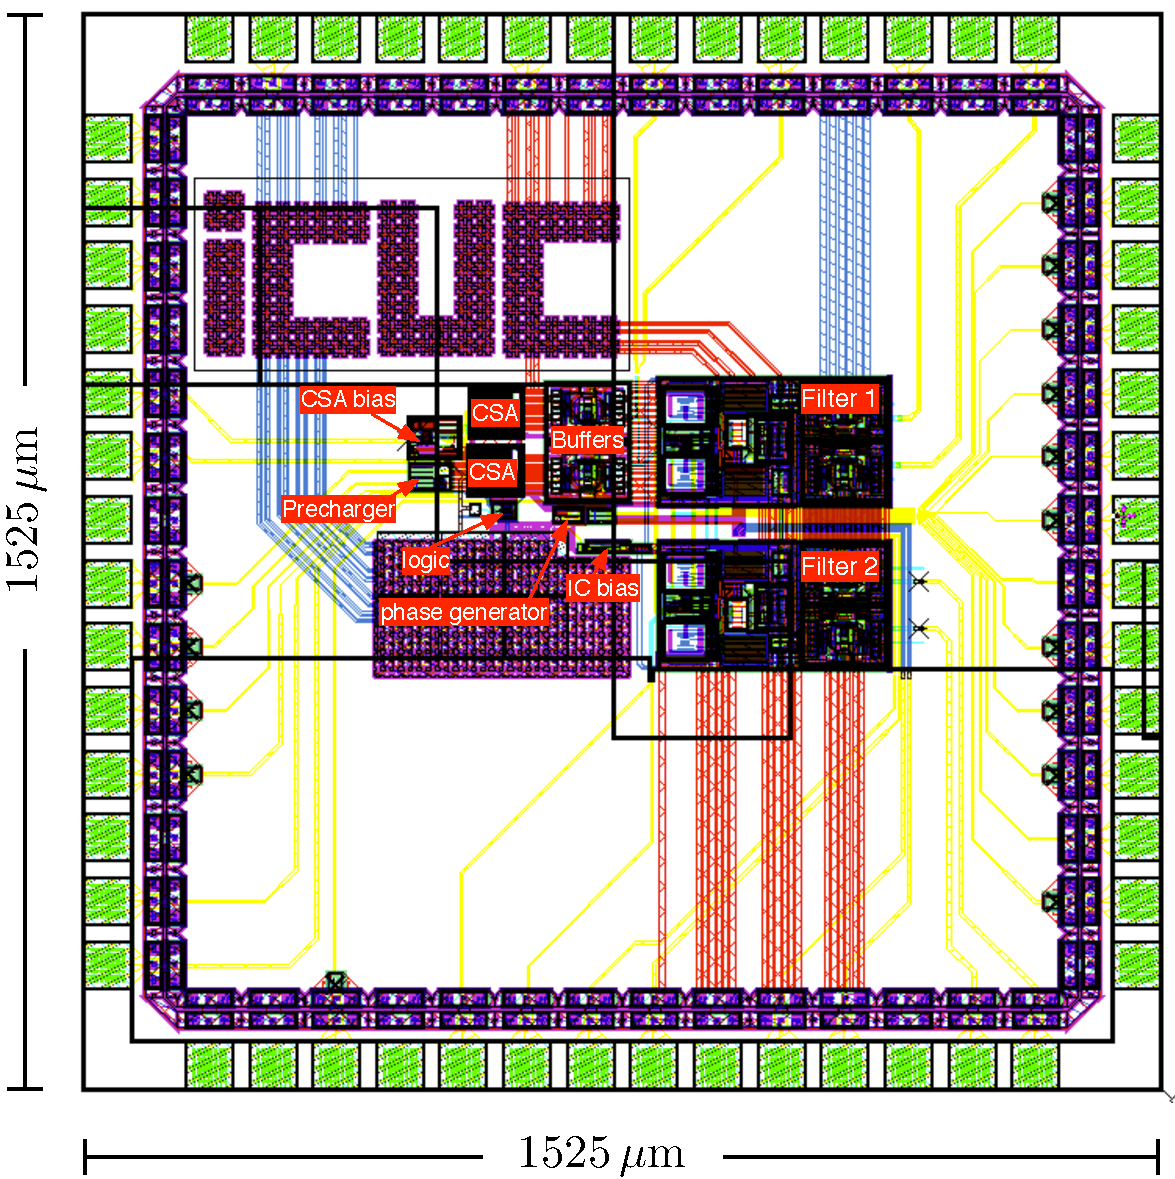
\includegraphics[width=0.5\textwidth]{./figures/theorical/IC_layout}
%	\caption{\label{layout}The Bean V2 prototype layout.}
%\end{figure}

El esquema de la estructura general del circuito implementado por el IC se entrega en la figura \ref{thebean}. La primera etapa del IC consiste en un amplificador CSA, el cual se encarga de recibir la señal de entrada desde el detector y  generar un escalón de voltaje proporcional a la cantidad de carga inyectada. Junto con el amplificador, esta etapa cuenta con: un bloque destinado a generar la polarización del amplificador; un bloque para el control de la red de \textit{feedback}, que permite seleccionar la capacitancia de realimentación dependiendo del modo de operación; y por último, cuenta con un bloque de pre-carga para inyectar carga en la entrada con el objetivo de mover el \textit{baseline}\footnote{El baseline se define como el valor de la salida de un CSA cuando no se presenta estímulo en la entrada.} del CSA a un punto que optimice el rango de salida. En el IC también existe un segundo bloque CSA idéntico al anterior, con la diferencia de que posee la salida y la entrada conectadas, esto con el objetivo de poder generar y medir el \textit{baseline}.
	


%\begin{figure}[!t]
%	% XCircuit output "tx_ltspice.tex" for LaTeX input from tx_ltspice.eps
\def\putbox#1#2#3#4{\makebox[0in][l]{\makebox[#1][l]{}\raisebox{\baselineskip}[0in][0in]{\raisebox{#2}[0in][0in]{\scalebox{#3}{#4}}}}}
\def\rightbox#1{\makebox[0in][r]{#1}}
\def\centbox#1{\makebox[0in]{#1}}
\def\topbox#1{\raisebox{-0.60\baselineskip}[0in][0in]{#1}}
\def\midbox#1{\raisebox{-0.20\baselineskip}[0in][0in]{#1}}
\begin{center}
\scalebox{0.4}{
   \normalsize
   \parbox{17in}{
   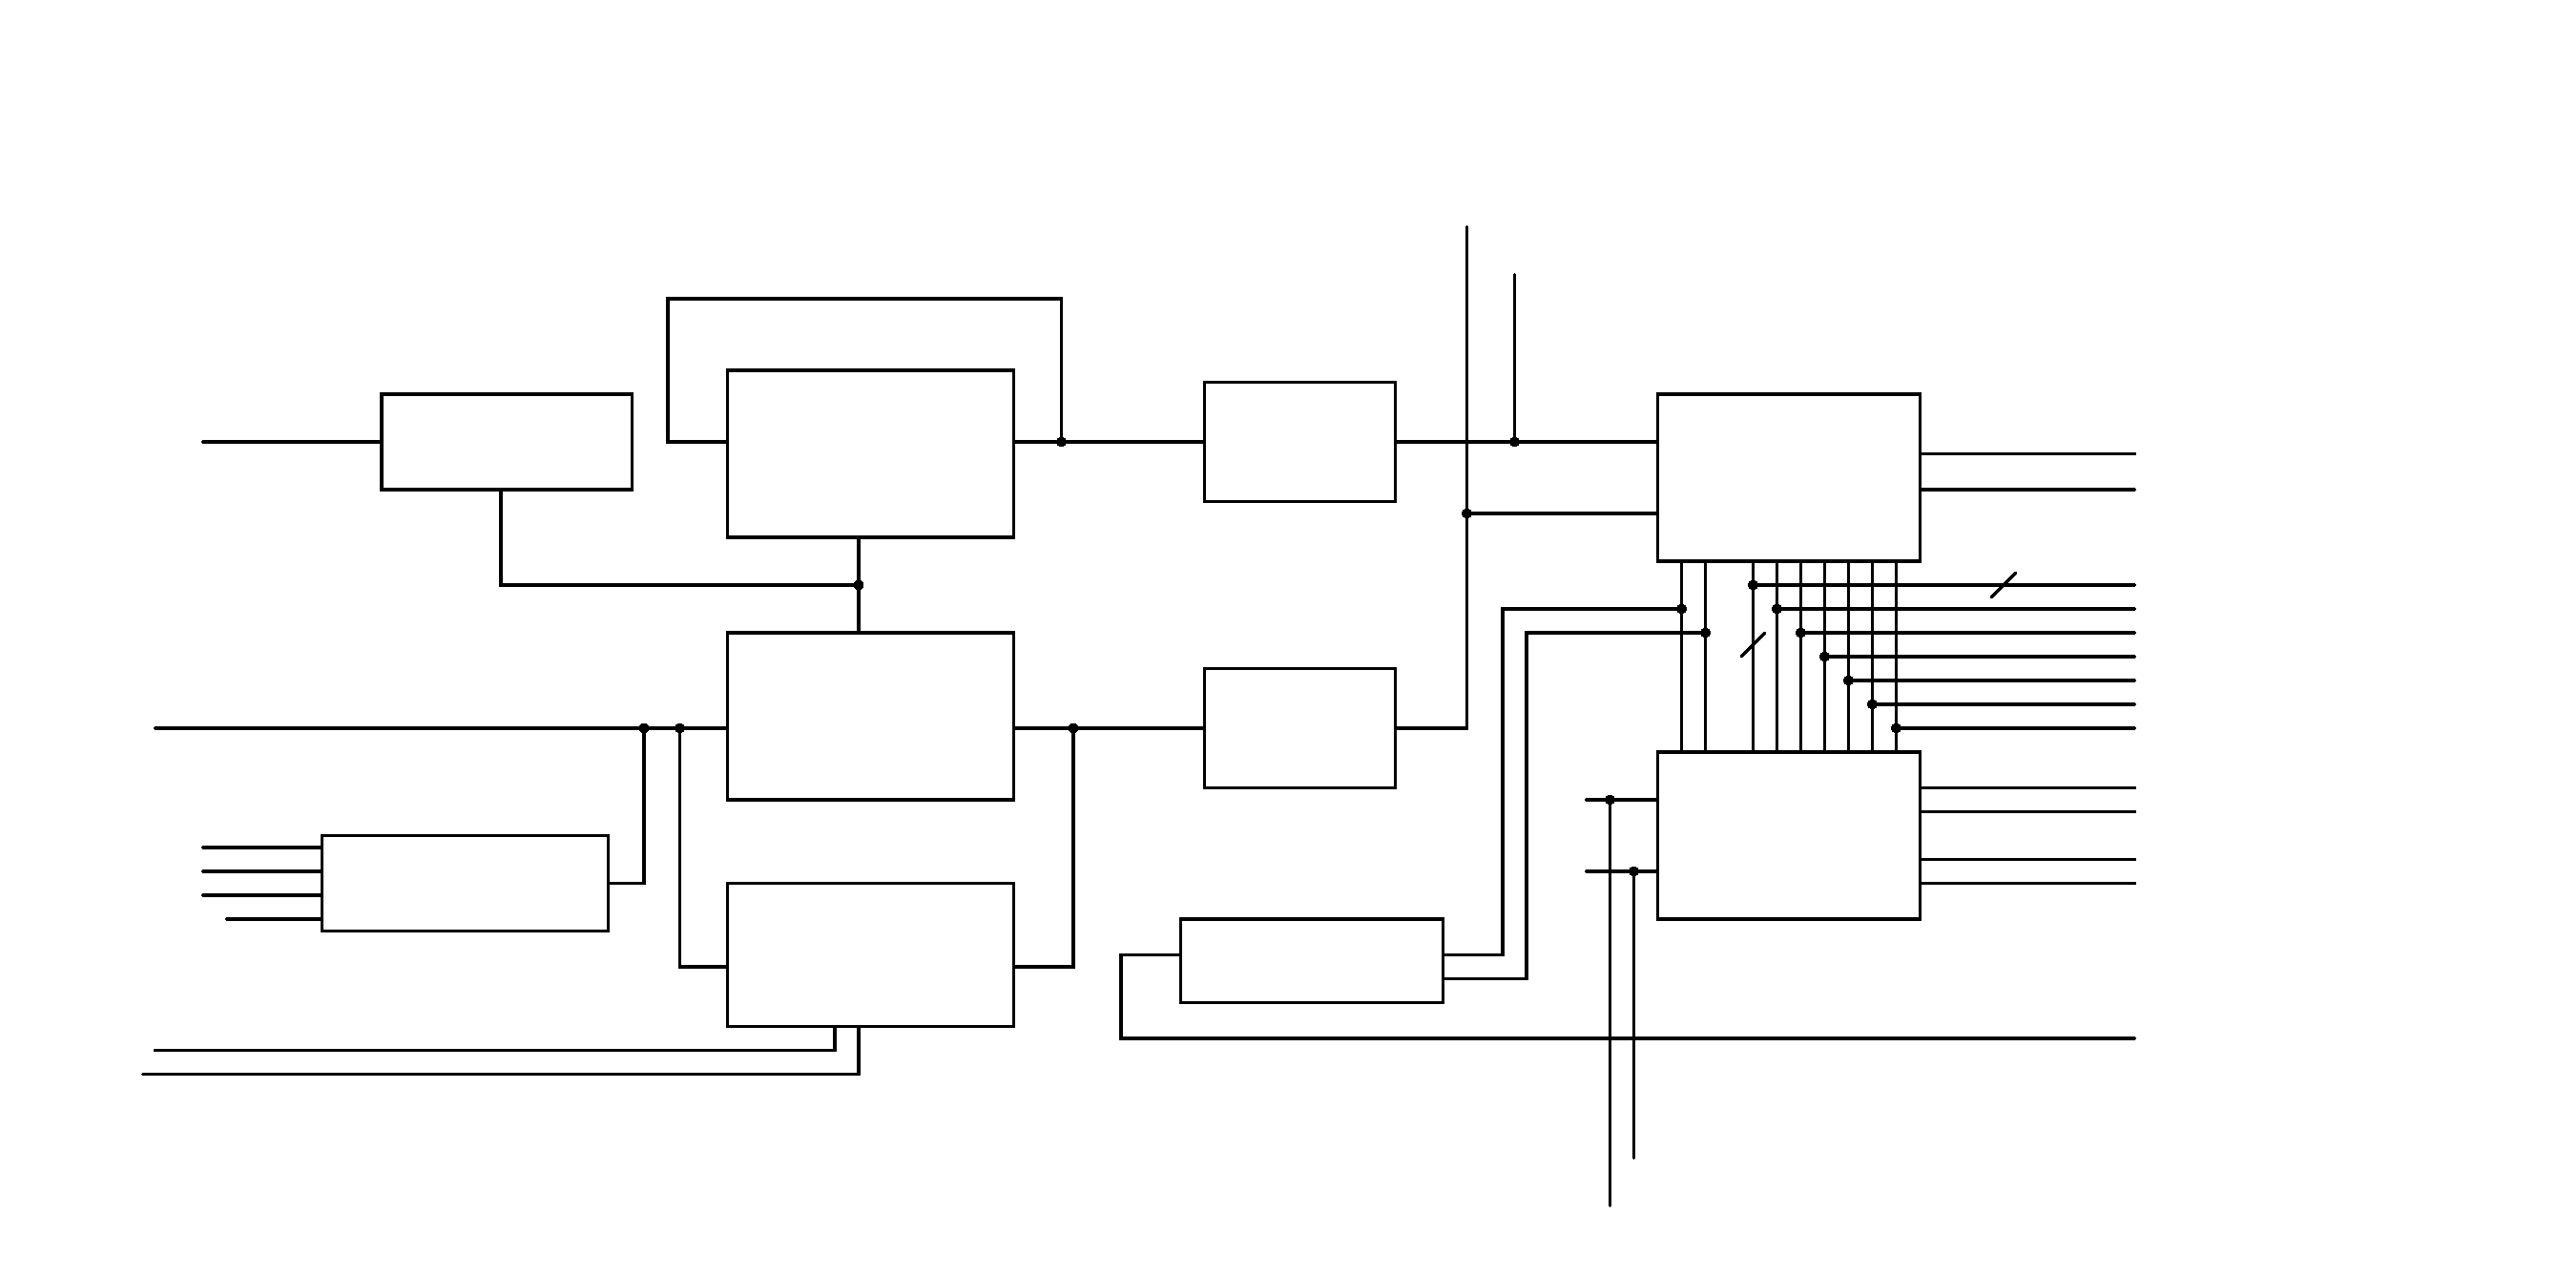
\includegraphics[scale=1]{./figures/theorical/thebeanv2.eps}\\
% translate x=1296 y=1280 scale 0.38
\putbox{0.06in}{5.72in}{1.2}{res\_bias\_ext}%
\putbox{0.06in}{3.72in}{1.2}{Vin\_csa}%
\putbox{0.06in}{2.89in}{1.2}{Vref\_prechar}%
\putbox{0.06in}{2.72in}{1.2}{clk\_prechar1}%
\putbox{0.06in}{2.56in}{1.2}{clk\_prechar2}%
\putbox{0.06in}{2.39in}{1.2}{C\_ext\_prechar}%
\putbox{0.06in}{1.47in}{1.2}{op\_mode}%
\putbox{0.06in}{1.31in}{1.2}{rst\_csa}%
\putbox{2.72in}{5.64in}{1.2}{CSA\_bias}%
\putbox{2.31in}{2.64in}{1.2}{pre\_charger}%
\putbox{5.31in}{2.22in}{1.2}{CSA\_ctrl}%
\putbox{5.31in}{1.89in}{1.2}{feedback}%
\putbox{5.56in}{5.56in}{1.2}{CSA}%
\putbox{5.56in}{3.72in}{1.2}{CSA}%
\putbox{8.56in}{5.64in}{1.2}{buffer}%
\putbox{8.56in}{3.64in}{1.2}{buffer}%
\putbox{8.31in}{2.06in}{1.2}{phase\_gen}%
\putbox{11.97in}{5.39in}{1.2}{Filter}%
\putbox{11.97in}{2.89in}{1.2}{Filter}%
\putbox{14.97in}{4.72in}{1.2}{CS\_Bx}%
\putbox{14.97in}{4.56in}{1.2}{out\_s}%
\putbox{14.97in}{4.39in}{1.2}{Vocm}%
\putbox{14.97in}{4.22in}{1.2}{hold}%
\putbox{14.97in}{4.06in}{1.2}{rst}%
\putbox{14.97in}{3.89in}{1.2}{sgn}%
\putbox{14.97in}{3.72in}{1.2}{Vicm}%
\putbox{14.97in}{5.64in}{1.2}{Vo+\_ch}%
\putbox{14.97in}{5.39in}{1.2}{Vo-\_ch}%
\putbox{14.97in}{3.31in}{1.2}{Vo-\_fil}%
\putbox{14.97in}{3.14in}{1.2}{Vo+\_fill}%
\putbox{14.97in}{2.81in}{1.2}{Vo-\_bp\_fill}%
\putbox{14.97in}{2.64in}{1.2}{Vo+\_bp\_fill}%
\putbox{14.97in}{1.56in}{1.2}{clk}%
\putbox{11.31in}{0.39in}{1.2}{Vin-\_fill}%
\putbox{11.14in}{0.06in}{1.2}{Vin+\_fill}%
\putbox{10.14in}{7.39in}{1.2}{Vout\_csa}%
\putbox{10.47in}{7.06in}{1.2}{baseline}%
   } % close 'parbox'
   } % close 'scalebox'
\end{center}

%	\caption{\label{thebean}The Bean V2 prototype layout.}
%\end{figure}

Ambas salidas tanto la del CSA como la del \textit{baseline} pasan por respectivos \textit{buffers}. Las salidas de ambos \textit{buffer} están disponibles para ser leídas en respectivos pines del integrado. Posteriormente ambas señales sirven de entrada para el filtro.

El filtro es implementado por un integrador totalmente diferencial de capacitores conmutados con capacitancia configurable por medio de señales digitales. Además cuenta con cuatro señales de control que permiten configurar el modo de operación controlando: el \textit{clock} de conmutación, el signo de la entrada del filtro, la procedencia de la señal de salida (la cual puede provenir desde la entrada o desde la salida del filtro), y la opción de poder mantener la señal a la salida con el fin de facilitar la lectura. Además el filtro necesita dos voltajes de referencia para fijar los valores de modo común tanto para la entrada como para la salida.
	Por último, existe una segunda versión del filtro para propósitos de pruebas y caracterización. Esta versión del filtro cuenta con las entradas conectadas directamente a pines del integrado, y comparte las señales de control y la polarización con el filtro antes mencionado.
	
 	
	

\section{Detalle del integrado}
 

\subsection{El CSA}

El objetivo de este bloque es convertir la carga generada por el detector en una señal de voltaje. La figura \ref{csa} muestra en detalle la forma en que es implementado dentro del IC. 

\begin{figure}[!h]
	\centering
	% XCircuit output "tx_ltspice.tex" for LaTeX input from tx_ltspice.eps
\def\putbox#1#2#3#4{\makebox[0in][l]{\makebox[#1][l]{}\raisebox{\baselineskip}[0in][0in]{\raisebox{#2}[0in][0in]{\scalebox{#3}{#4}}}}}
\def\rightbox#1{\makebox[0in][r]{#1}}
\def\centbox#1{\makebox[0in]{#1}}
\def\topbox#1{\raisebox{-0.60\baselineskip}[0in][0in]{#1}}
\def\midbox#1{\raisebox{-0.20\baselineskip}[0in][0in]{#1}}
\begin{center}
\scalebox{0.4}{
\normalsize
\parbox{9in}{
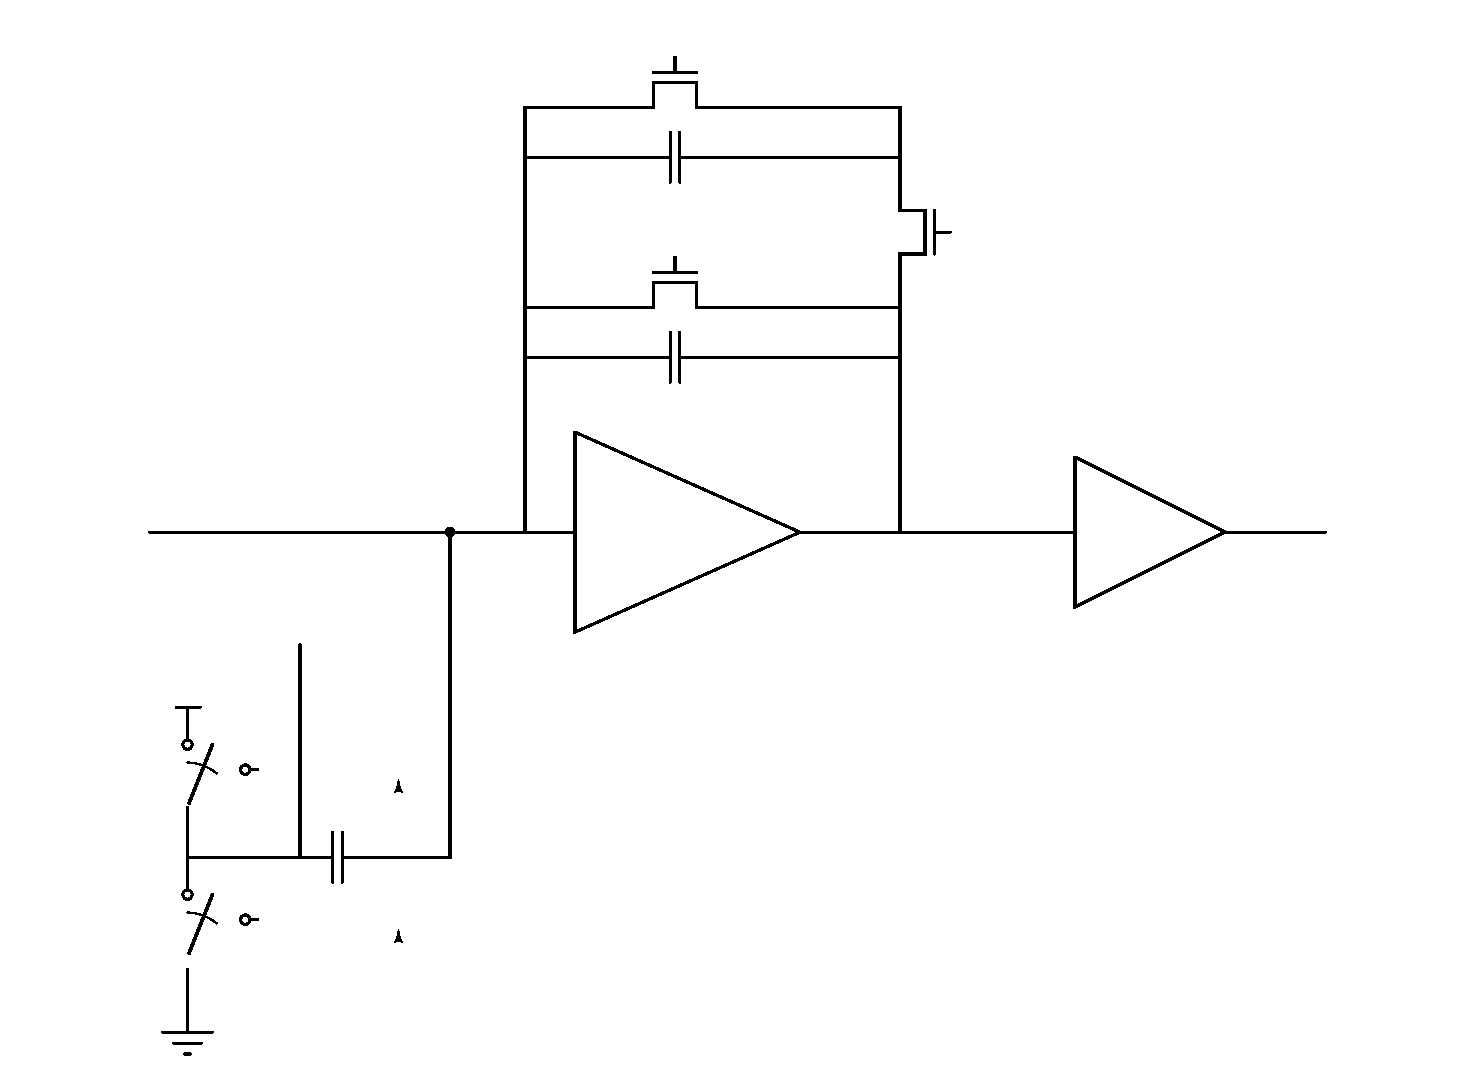
\includegraphics[scale=1]{./figures/theorical/csa_circuit2.eps}\\
% translate x=1152 y=860 scale 0.38
\putbox{0.22in}{3.62in}{1.2}{Vin\_csa}%
\putbox{0.72in}{2.45in}{1.2}{Vref\_pc}%
\putbox{1.56in}{2.87in}{1.2}{Cext\_pc}%
\putbox{4.06in}{5.54in}{1.2}{rst\_csa}%
\putbox{4.14in}{6.79in}{1.2}{rst\_csa}%
\putbox{6.39in}{5.54in}{1.2}{op\_mode}%
\putbox{8.72in}{3.62in}{1.2}{Vout\_csa}%
\putbox{0.14in}{1.87in}{1.2}{$\phi_1$\_pc}%
\putbox{0.06in}{1.04in}{1.2}{$\phi_2$\_pc}%
 } % close 'parbox'
 } % close 'scalebox'
\vspace{-\baselineskip} % this is not necessary, but looks better
\end{center}

	\caption{\label{csa}The Bean V2 prototype layout.}
\end{figure}

El CSA cuenta con dos condensadores de realimentación los cuales permiten configurar el valor de la capacitancia de realimentación $C_F$, por medio de la señal digital \verb+op_mode+. Así $C_F= C_{Cal}$ en el modo DCal y $C_F= C_{Cal}+ C_{Op}$ en el modo SDT. De este modo, es posible implementar distintas ganancias para los diferentes modos de operación. Por otro lado, la señal \verb+rst_csa+ permite implementar la función de \textit{reset} en la red de realimentación descargando la carga almacenada en los condensadores.

 Debido a la configuración con la cual fue implementado el CSA, el baseline se establecerá aproximadamente a $V_T$ o $0.5V$, sin embargo, la región de operación de alta ganancia se encuentra aproximadamente a los $0.4V$ de los rieles. Para solucionar este problema es que el CSA cuenta con circuito de pre-carga, el cual inyecta una cantidad conocida de carga para mover el baseline más cerca de los $0.4V$.
 

\subsection{Pre-charger}


El circuito de pre-carga fue diseñado para inyectar carga a la entrada del CSA con el objetivo de ajustar el baseline y a la vez para cumplir con propósitos de calibración.
 En la imagen \ref{Cir_vin} se muestra una versión simplificada del circuito. Esta formado por dos switches implementados con transistores y un condensador $C_{PC}$ el cual esta conectado a la entrada del CSA. Para cambiar el valor de la capacitancia de este condensador (modo SDT) existe la posibilidad de conectar un condensador externo en paralelo por medio de la señal \verb+cap_prechar_ext+.
 
 
La forma en que se controla el circuito de pr-ecarga se basa en dos señales de clock desfasadas no sobrepuestas. Cuando la primera señal esta activa ($\phi_1$), el extremo izquierdo del condensador queda conectado a un voltaje de referencia externo $V_{DD\_ref}$ configurable por medio de la señal \verb+V_ref_prechar+. Posteriormente, cuando la segunda señal esta activa ($\phi_2$), el extremo izquierdo es conectada a tierra. En cada transición de $\phi_2$ a $\phi_1$ el condensador inyecta una carga de $Q_{CP}=C_{CP} \cdot V_{DD\_ref}$ en la entrada del CSA. Esto provoca una variación de voltaje en la salida de $\Delta V =-C_{CP} \cdot V_{DD\_ref}/C_F$, en donde $C_F$ es la capacitancia de realimentación. La inyección de carga se realiza justo después de que el CSA es habilitado, reduciendo el voltaje de baseline a la salida. 

\begin{figure}
\def\putbox#1#2#3{\makebox[0in][l]{\makebox[#1][l]{}\raisebox{\baselineskip}[0in][0in]{\raisebox{#2}[0in][0in]{#3}}}}
\def\rightbox#1{\makebox[0in][r]{#1}}
\def\centbox#1{\makebox[0in]{#1}}
\def\topbox#1{\raisebox{-\baselineskip}[0in][0in]{#1}}
\def\midbox#1{\raisebox{-0.5\baselineskip}[0in][0in]{#1}}
\begin{flushleft}
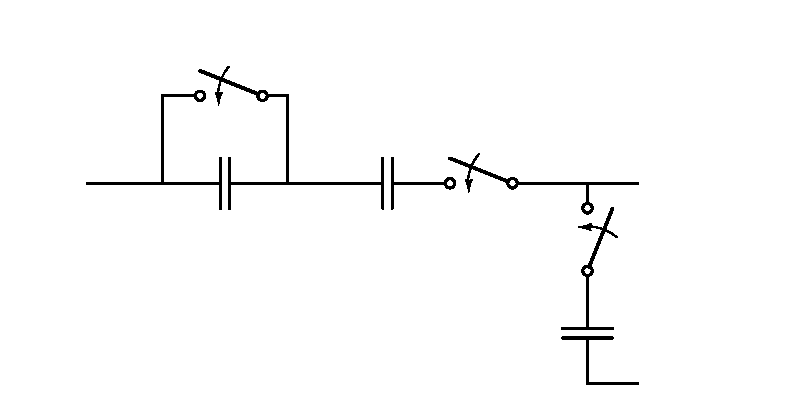
\includegraphics[width=1\textwidth]{./figures/theorical/Injector_de_carga.eps}\\
% translate x=816 y=166 scale 0.38
\putbox{0.06in}{1.42in}{Vin}%
\putbox{1.22in}{2.34in}{JP9}%
\putbox{1.22in}{1.00in}{C36}%
\putbox{1.22in}{0.75in}{0.5pF}%
\putbox{2.31in}{1.00in}{C37}%
\putbox{2.31in}{0.75in}{27pF}%
\putbox{2.81in}{1.75in}{JP10}%
\putbox{4.22in}{1.42in}{Vin\_csa}%
\putbox{4.22in}{0.09in}{Cext\_pc}%
\putbox{3.14in}{0.50in}{C38}%
\putbox{3.14in}{0.25in}{25pF}%
\putbox{3.22in}{1.00in}{JP11}%
\end{flushleft}
\caption{\label{Cir_vin}Circuito de inyección de carga en la tarjeta, para simular un detector.}
\end{figure}

\subsection{Filtro}
La segunda gran etapa del integrado corresponde a un filtro, el cual posee la ventaja de poder implementar funciones de peso arbitrarias, permitiendo de este modo, generar filtros que maximicen la SNR ayudando a reducir el ruido del proceso de lectura tal como se describe en Avila er al 2013. Este filtro es un prototipo para the Bean V2.

Con el objetivo de generar funciones de peso arbitrarias, el filtro implementa la ecuación \ref{theorical:ecuacion_f_z}, por medio de un integrador de capacitores conmutados totalmente diferencial. El esquema general de este circuito se puede apreciar en la figura \ref{theorical:filtro}.

El filtro posee dos fases de operación. Durante la primera fase, $\phi_1$, ocurre el muestreo,  la diferencia de voltaje de la entrada  carga ambos capacitores $C_S$. Durante la segunda fase, $\phi_2$, el cortocircuito virtual de la entrada del OTA fuerza a que la carga almacenada en $C_S$ sea transferida hacia el capacitor $C_F$. De este modo, el voltaje en la salida al final de la segunda fase es igual al voltaje en la iteración anterior más $C_S \Delta V_i^k / C_F$. De este modo la ganancia del filtro es proporcional a la razón entre las capacitores $C_S$ y $C_F$.
 
La capacitancia $C_S$ es implementada por un conjunto de capacitores en paralelo que pueden conectarse por medio de switches. De este modo, es posible cambiar digitalmente el valor de la capacitancia $C_S$. Esto último permite implementar una ganancia configurable digitalmente. Las señales \verb+CSB0+ a \verb+CSB5+ realizan el control digital de los respectivos capacitores.

El filtro también cuenta con un grupo de señales que permiten configurar su operación. El multiplexor de entrada permite intercambiar las señales de entrada, permitiendo controlar el sentido de la integración, lo cual es utilizado para implementar las pendientes negativas de las funciones de peso\footnote{Denominado CDS}. El multiplexor de salida, por otro lado, permite evitar el filtro en caso de que se estime necesario para STD mode o para modos de calibración. También cuenta con una señal de \textit{reset} que permite desaguar la carga de los capacitores $C_S$ y $C_F$. Posee una señal para mantener la salida en estado de \textit{hold} con propósito de facilitar mediciones. 

El OTA cuenta con una red interna de control de modo común de salida(CMFB). Tanto los voltajes de modo común de entrada como el de salida quedan quedan disponibles para ser ajustados por referencias externas. 
 



\begin{equation}
F(z)= \sum_{j=0}^{N-1} a_{N-j}z^{-1}
\label{theorical:ecuacion_f_z}
\end{equation}

\begin{figure}[!h]
	\centering
	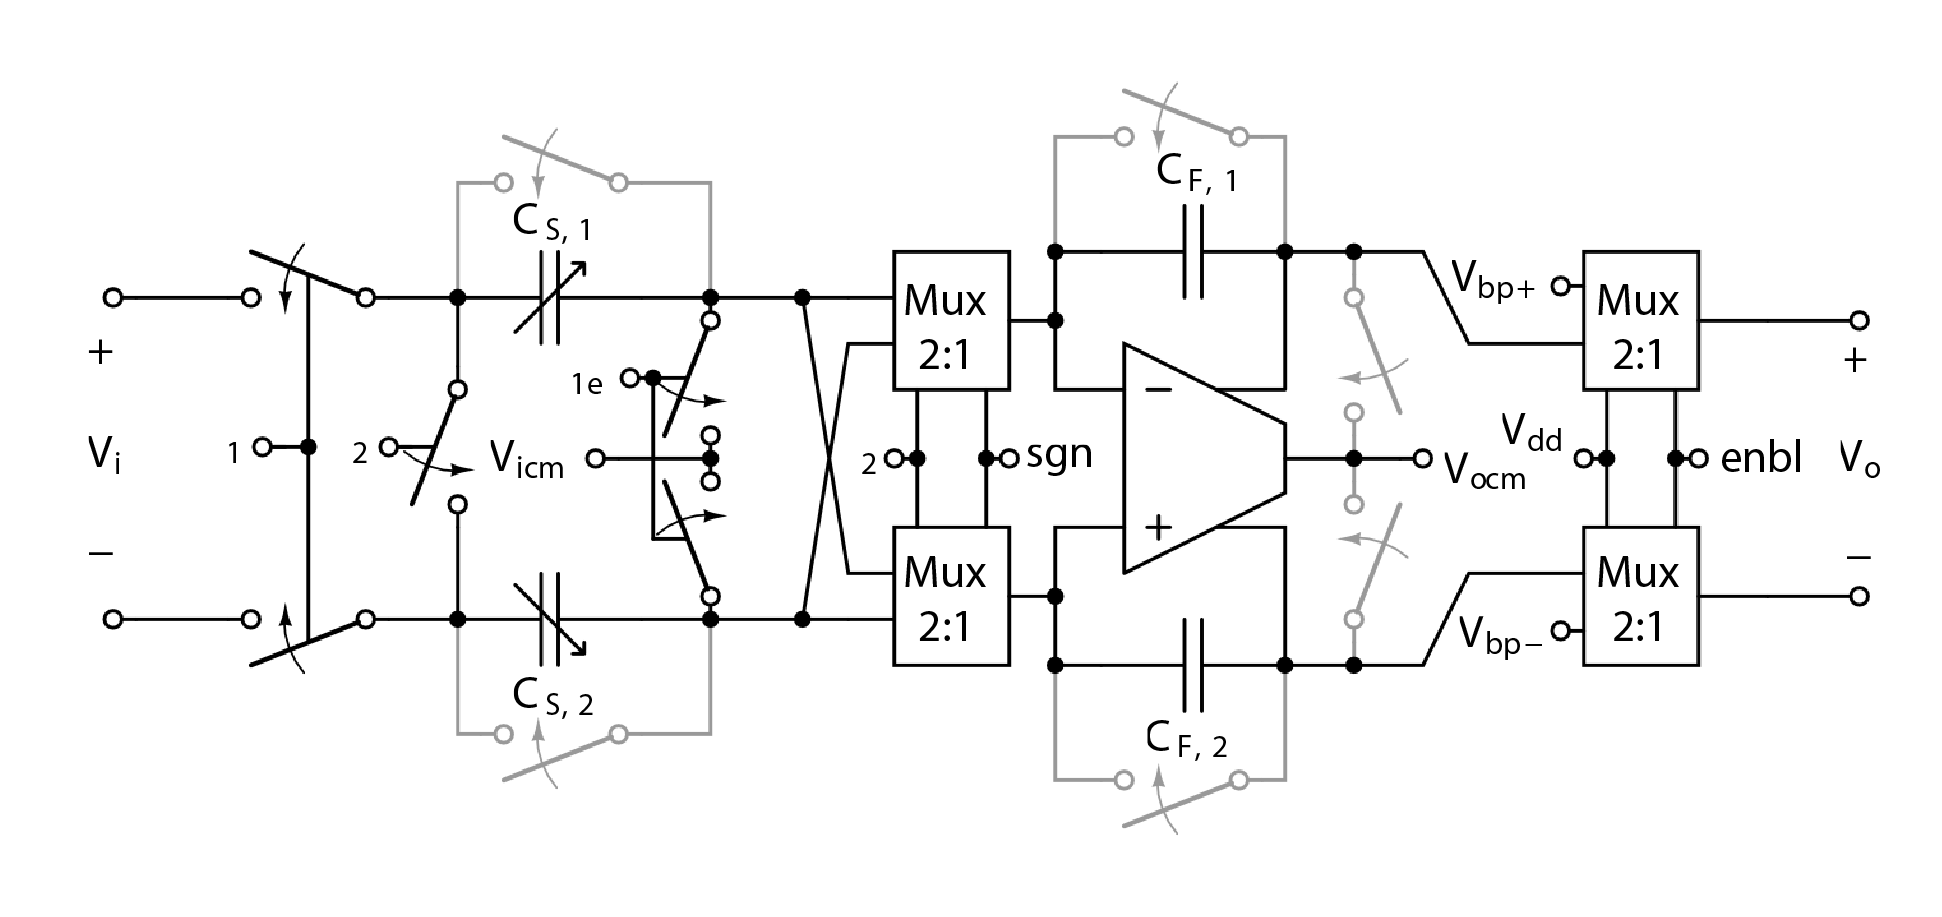
\includegraphics[width=1\textwidth]{./figures/theorical/filtro.png}
	\caption{\label{theorical:filtro}The Bean V2 prototype layout.}
\end{figure}

\section{Pruebas y diagramas de tiempo}





\subsection{Diagramas de tiempo}
\begin{figure}[!t]
	\centering
	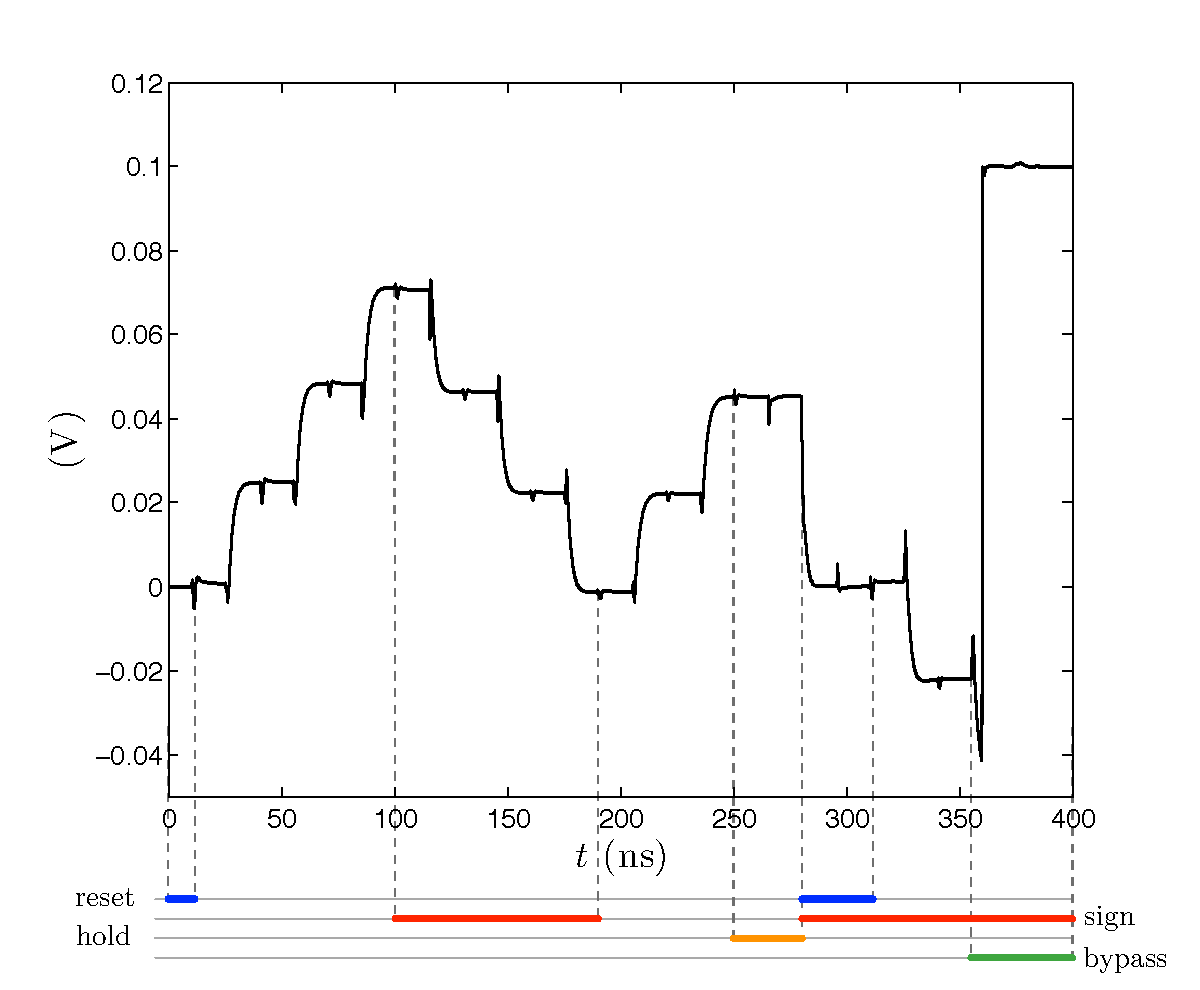
\includegraphics[width=5in]{./figures/theorical/test_filter_after_omni.eps}
	\caption{Filter functionality simulation. $V_\textit{in}=0.1\,V$ and $\text{gain}=0.25\,V/V$.}\label{fig:test_filter_after_omni}
\end{figure}

\begin{figure}[!t]
	\centering
	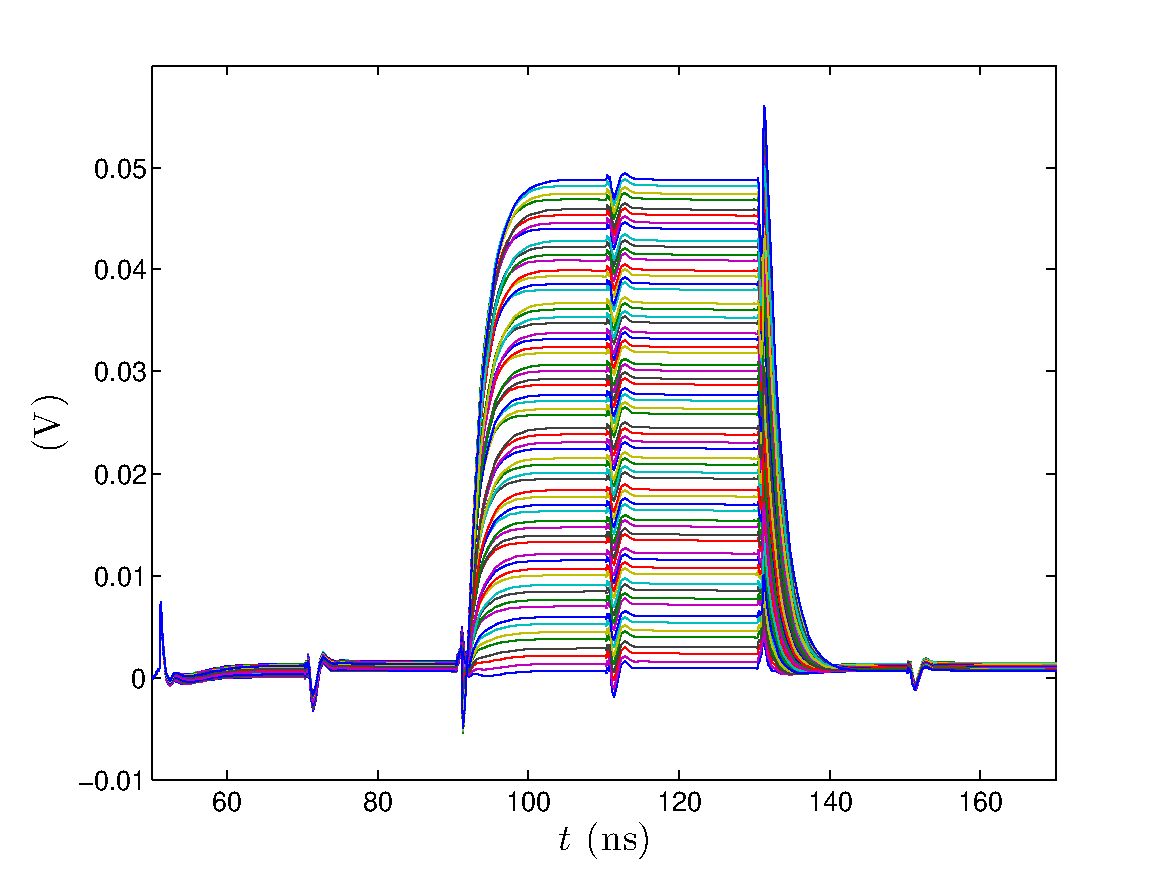
\includegraphics[width=4.4in]{./figures/theorical/gain_curves.pdf}
	\caption[Filter step response for constant input for the 64 possible programmable gains.]{Filter step response for constant input for the 64 possible programmable gains. \mbox{$V_\textit{in}=0.1\,V$} and \mbox{$T_s=40\,\text{ns}$}.}\label{fig:gain_curves}
\end{figure}

\begin{figure}[!t]
	\centering
	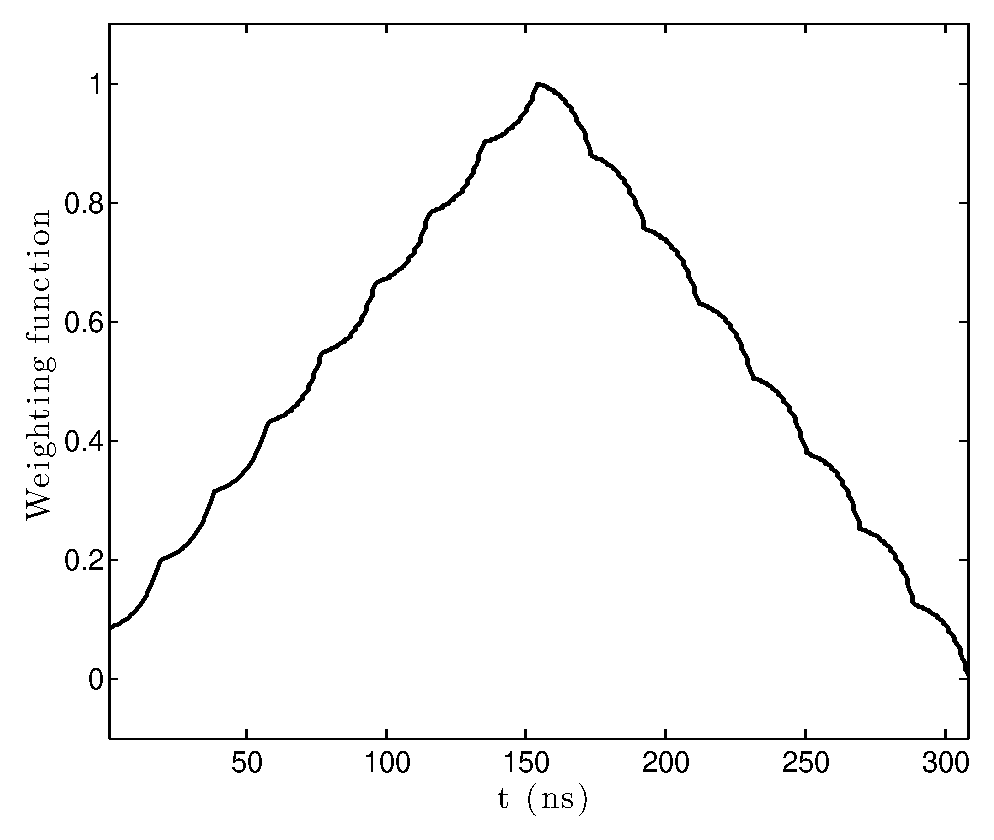
\includegraphics[width=3.6in]{./figures/theorical/sim_wf}
	\caption{SPICE-simulated weighting function. $\tau=8\,\text{ns}$, $N=16$ and $T_s=19.25\,\text{ns}$.}\label{fig:sim_wf}
\end{figure}

\subsection{Diseño de pruebas}

\begin{figure}[!t]
	\centering
	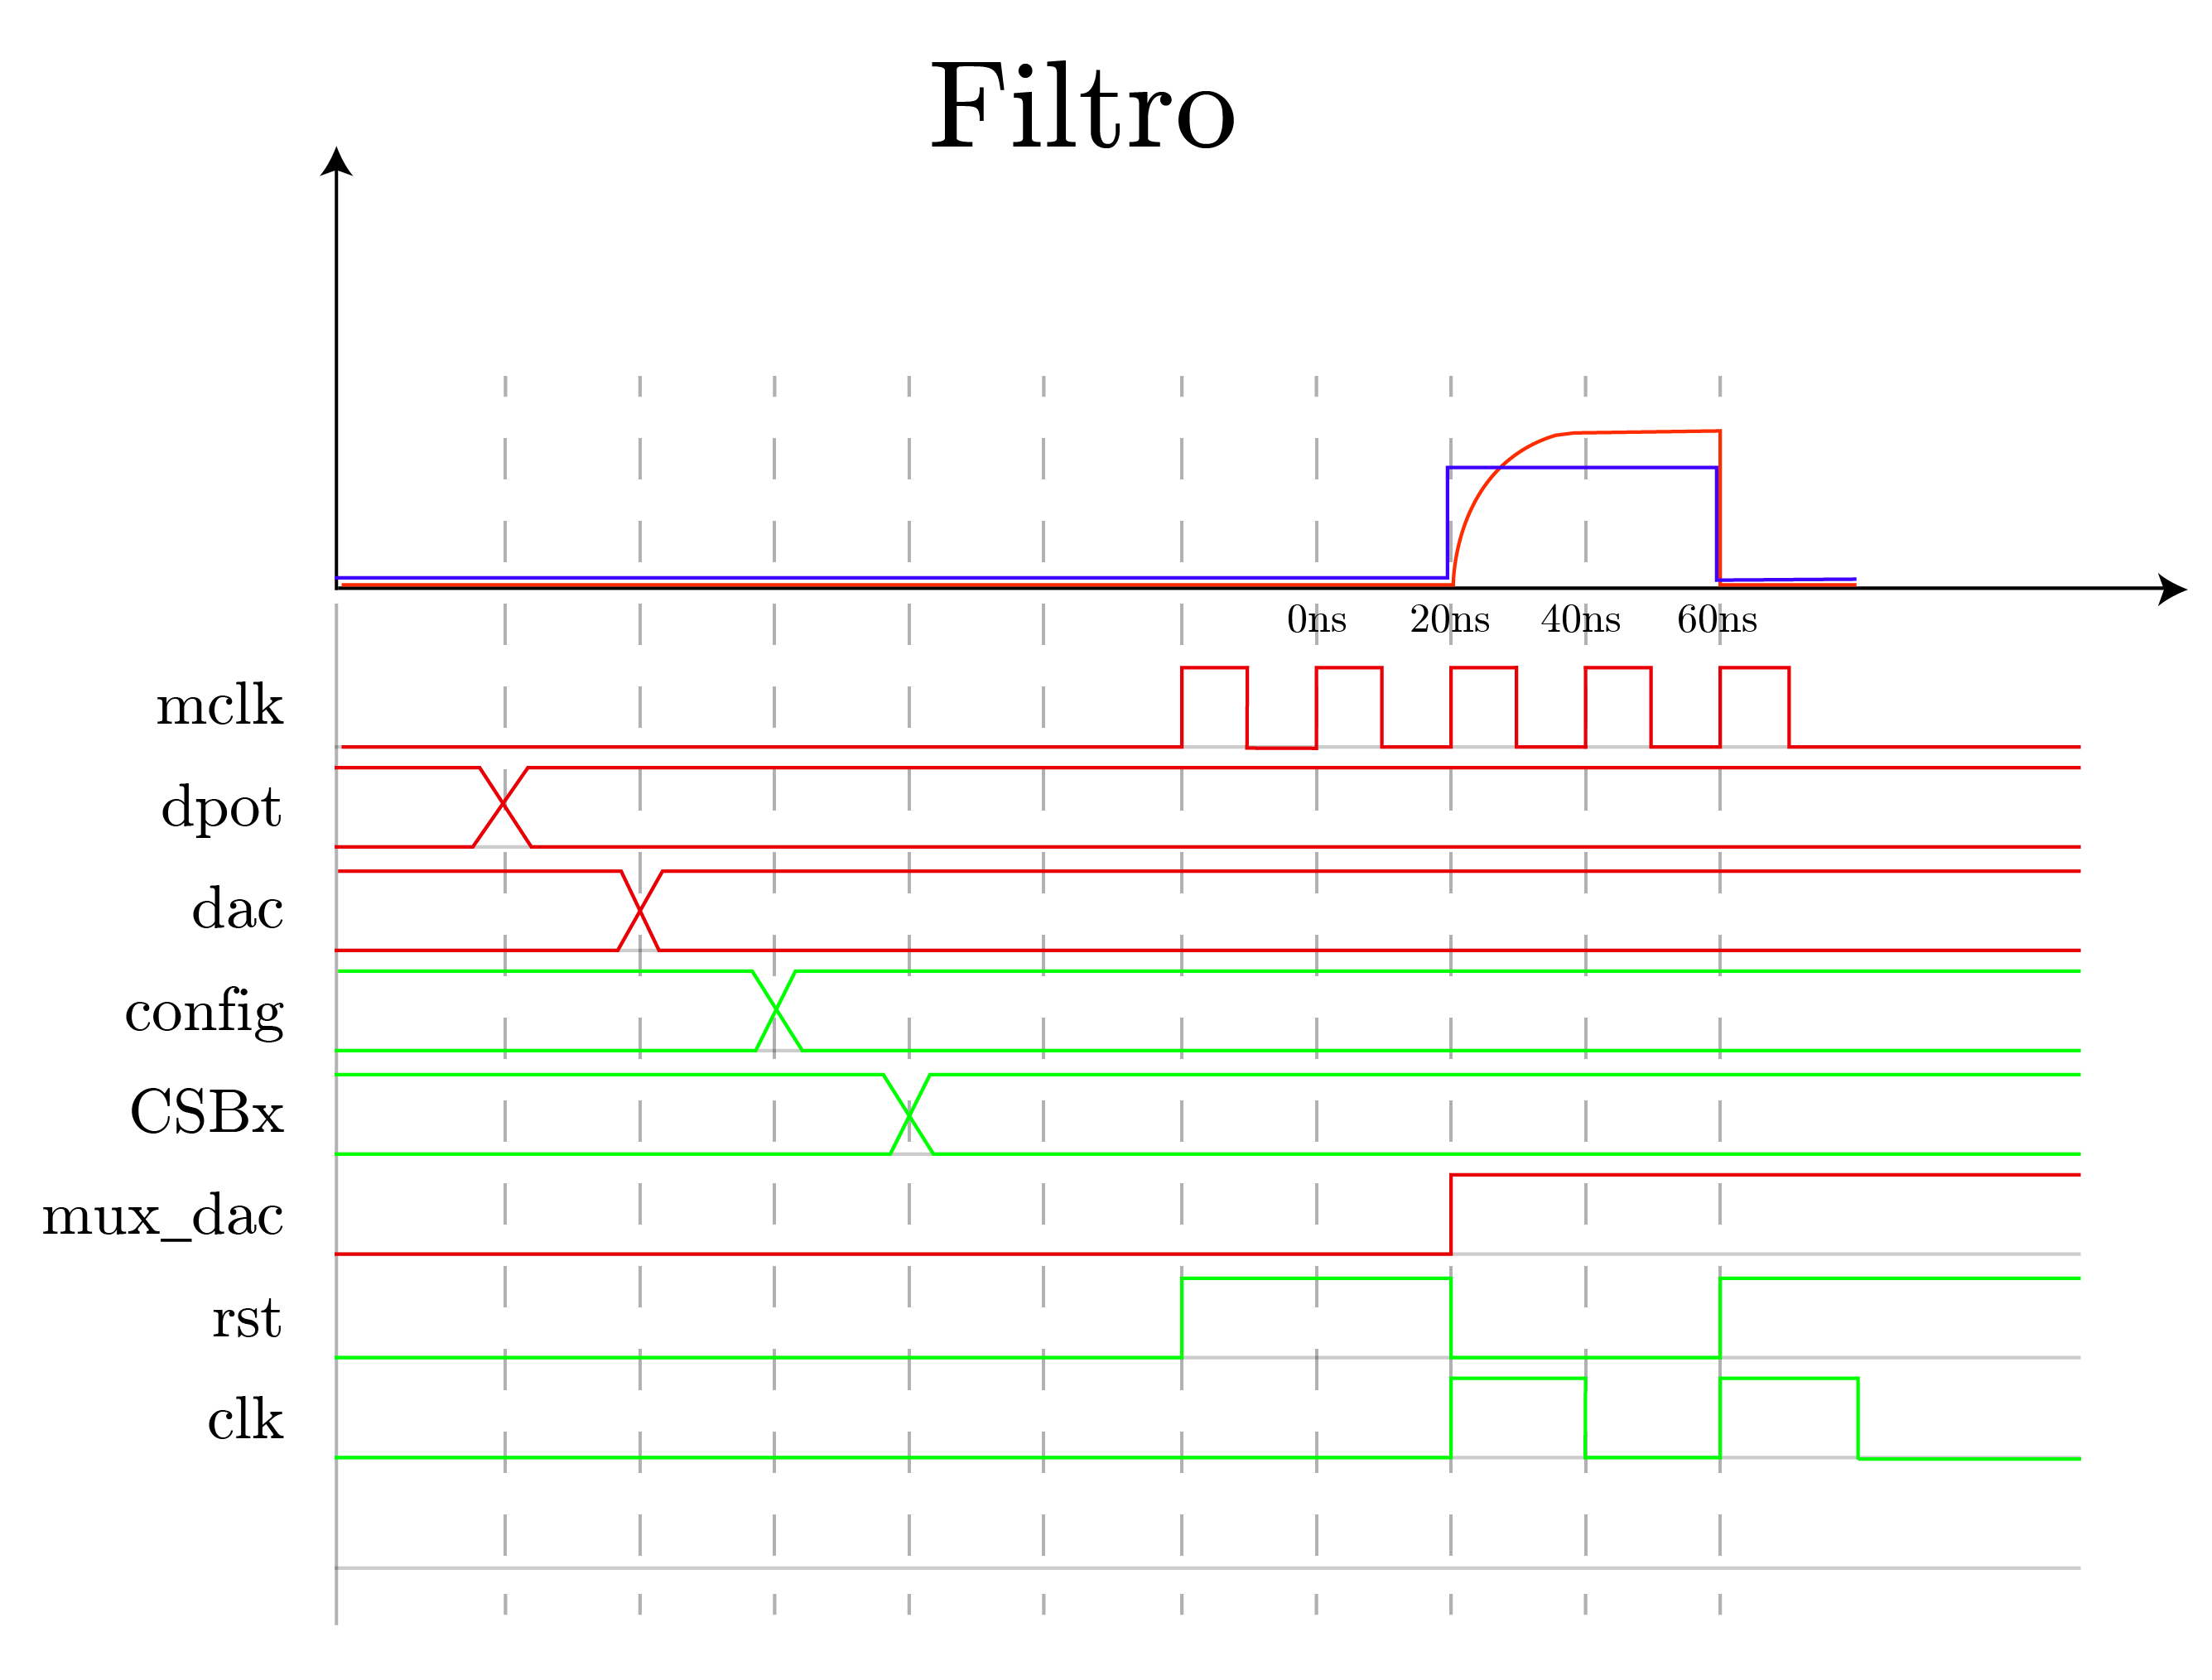
\includegraphics[width=1\textwidth]{./figures/theorical/tiempos_filtro.png}
	\caption{Diagrama de señales para las pruebas realizadas al filtro .}\label{fig:diagramafiltro}
\end{figure}

\begin{figure}[!t]
	\centering
	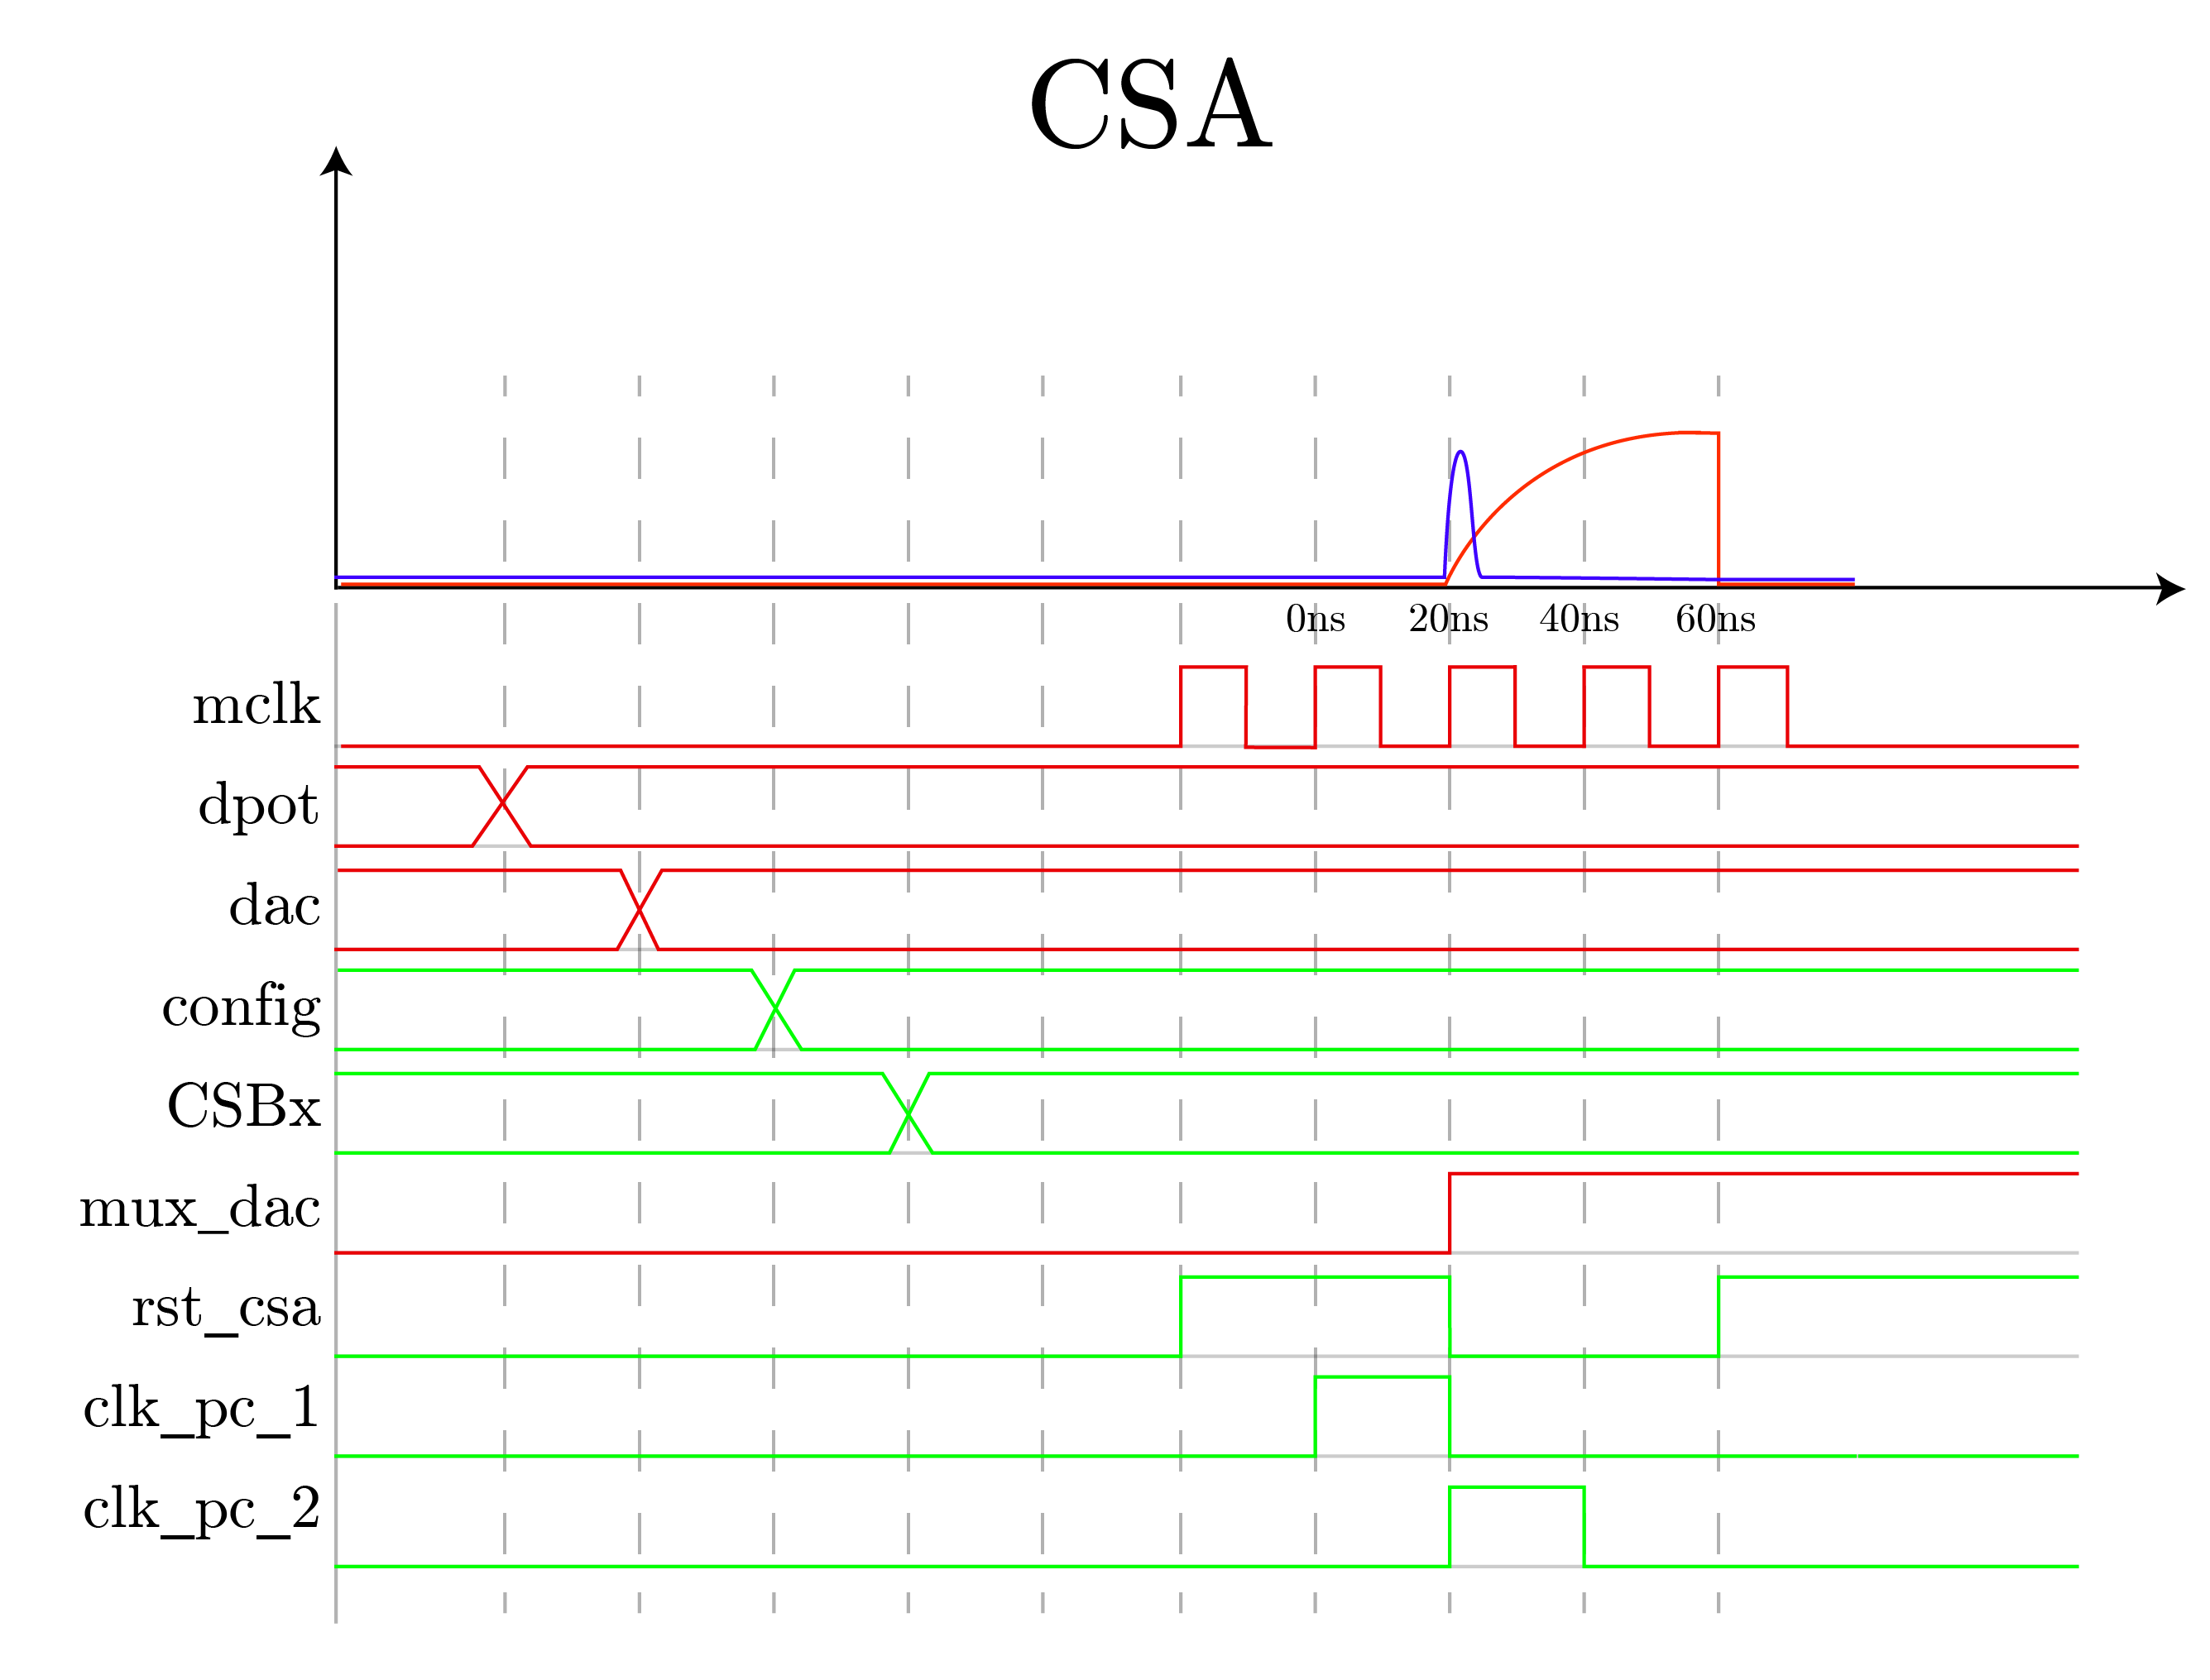
\includegraphics[width=1\textwidth]{./figures/theorical/tiempos_csa.png}
	\caption{Diagrama de señales para las pruebas realizadas al CSA.}\label{fig:diagramacsa}
\end{figure}



